\documentclass[12pt]{article}

\usepackage{amsmath}
\usepackage{amssymb}
\usepackage{enumitem}

\usepackage{tikz}
\usetikzlibrary{
    arrows.meta,
    calc,
    angles,
    quotes,
    decorations.pathmorphing
}
\usepackage[american]{circuitikz}


\setlist[enumerate,1]{label=\arabic*.}

\begin{document}

\begin{enumerate}

%=========================================================
\item
A wedge of mass $M$ is placed on a perfectly smooth horizontal surface. 
An inclined plane of angle $\theta$ is carved on its surface. A block of mass $m$ is attached to the wedge through a light spring of force constant $k$ placed along the incline. 
Initially the block is held at rest after compressing the spring by an amount $x$ relative to its natural length. 
After release, the block executes oscillatory motion relative to the wedge while the wedge recoils freely on the horizontal surface due to momentum conservation. 
Neglect any friction and assume the spring always remains along the incline. Determine the maximum horizontal velocity attained by the wedge during the motion.

\begin{center}
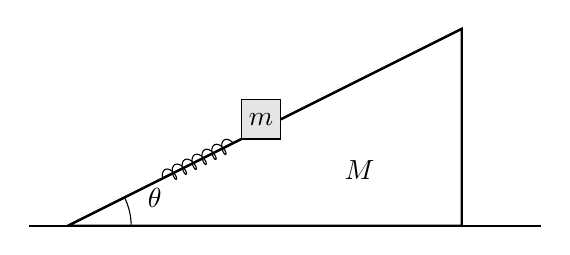
\begin{tikzpicture}[scale=1]

% Ground
\draw[thick] (-0.5,0) -- (6,0);

% Wedge
\draw[thick] (0,0) -- (5,0) -- (5,2.5) -- cycle;
\draw[thick] (0,0) -- (5,2.5);

% Angle theta
\draw (0.8,0) arc (0:27:0.8);
\node at (1.1,0.35) {$\theta$};

% Block
\draw[fill=gray!20] (2.2,1.1) rectangle (2.7,1.6);
\node at (2.45,1.35) {$m$};

% Spring
\draw[decorate,decoration={coil,aspect=0.5,segment length=4pt}] 
(1.2,0.6) -- (2.2,1.1);

% Label wedge
\node at (3.7,0.7) {$M$};

\end{tikzpicture}
\end{center}


A) $\dfrac{m}{M+m}\sqrt{\dfrac{kx^2}{m}}$

B) $\dfrac{m}{M+m}\sqrt{\dfrac{2kx^2}{m}}$

C) $\dfrac{m}{M}\sqrt{\dfrac{kx^2}{m}}$

D) $\dfrac{m}{M+m}\sqrt{\dfrac{kx^2}{2m}}$

%=========================================================
\item

A charged particle of mass $m$ and charge $q$ moves with speed $v$ in a horizontal circular path of radius $R$ under the influence of a uniform magnetic field directed vertically upward. 
Simultaneously, the particle is subjected to a uniform gravitational field directed vertically downward. 
The particle’s plane of motion remains horizontal only if the vertical forces balance appropriately so that no helical motion develops. 
Assuming steady circular motion with constant speed, determine the minimum magnetic field required so that the particle does not acquire any vertical drift.

A) $\dfrac{mg}{qv}$

B) $\dfrac{mv}{qR}$

C) $\dfrac{m}{q}\sqrt{\dfrac{g}{R}}$

D) $\dfrac{mgR}{qv}$

%=========================================================
\item 
A uniform rigid rod of length $L$ and mass $m$ is pivoted smoothly at one end and initially held horizontal. 
A small conducting ring of mass $m$ is threaded on the rod and is free to slide without friction along its length. 
The system is placed in a uniform magnetic field perpendicular to the plane of motion such that induced effects do not alter mechanical energy. 
When released from rest, the rod rotates downward under gravity and the ring slides outward simultaneously due to the varying normal reaction. 
Find the speed of the ring relative to ground when it reaches the lower end of the rod.

\begin{center}
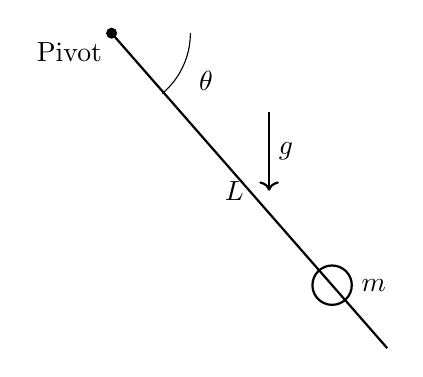
\begin{tikzpicture}[scale=1]

% Pivot
\fill (0,0) circle (2pt);
\node[below left] at (0,0) {Pivot};

% Rod at angle
\draw[thick] (0,0) -- (3.5,-4);

% Angle indicator (rotation)
\draw (1,0) arc (0:-50:1);
\node at (1.2,-0.6) {$\theta$};

% Ring on rod (near lower end)
\draw[thick] (2.8,-3.2) circle (0.25);
\node[right] at (3.05,-3.2) {$m$};

% Gravity arrow
\draw[->,thick] (2,-1) -- (2,-2);
\node[right] at (2,-1.5) {$g$};

% Length label
\node[left] at (1.8,-2) {$L$};

\end{tikzpicture}
\end{center}

A) $\sqrt{2gL}$

B) $\sqrt{gL}$

C) $\sqrt{\dfrac{4gL}{3}}$

D) $\sqrt{\dfrac{2gL}{3}}$

%=========================================================
\item

An ideal gas initially at pressure $P_0$ and volume $V_0$ undergoes a quasi-static process described by the relation 
\[
P = P_0\left(\dfrac{V_0}{V}\right)^n
\]
where $n$ is a real constant not equal to unity. The gas expands until its volume becomes $2V_0$. 
Assume the process is reversible and no heat losses occur other than those implied by the equation of state. 
Calculate the total work done by the gas during this process.

A) $\dfrac{P_0V_0}{n-1}\left(1-2^{1-n}\right)$

B) $P_0V_0\ln2$

C) $\dfrac{P_0V_0}{1-n}\left(2^{1-n}-1\right)$

D) $\dfrac{P_0V_0}{n}\left(2^{1-n}-1\right)$

%=========================================================
\item

A satellite of mass $m$ is moving in a nearly circular orbit of instantaneous radius $R$ around a planet of mass $M$. 
Due to extremely small atmospheric drag, the orbit slowly decays such that the radial distance decreases at a constant rate $\dfrac{dR}{dt}=-\alpha$, where $\alpha \ll v$. 
Assume the orbit remains quasi-circular at every instant. 
Determine the instantaneous rate of change of total mechanical energy of the satellite in terms of given parameters.

A) $\dfrac{GMm}{2R^2}\alpha$

B) $\dfrac{GMm}{R^2}\alpha$

C) $-\dfrac{GMm}{2R^2}\alpha$

D) $-\dfrac{GMm}{R^2}\alpha$

%=========================================================
\item

A capacitor of capacitance $C$ is initially charged to a potential difference $V$ and then connected to an ideal inductor $L$ forming an LC circuit. 
While oscillations are occurring, the separation between the plates of the capacitor is slowly increased such that the system remains electrically isolated and no radiation losses occur. 
Assuming the process is slow compared to oscillation time so that adiabatic invariants apply, determine how the maximum current attained in the circuit changes.

A) unchanged

B) increases

C) decreases

D) zero

%=========================================================
\item

A particle moves in a one-dimensional potential field described by 
\[
U(x)=\alpha x^4 - \beta x^2 + \gamma
\]
where $\alpha,\beta>0$. The particle is given total energy exactly equal to the potential barrier height separating the two minima. 
Near the unstable equilibrium point, the restoring force becomes very weak and motion slows dramatically. 
Determine the qualitative behaviour of the time period as the particle approaches the turning point.

A) finite

B) diverges logarithmically

C) proportional to amplitude

D) constant

%=========================================================
\item 

A circular conducting loop of radius $R$ rotates with constant angular velocity $\omega$ about a diameter in a uniform magnetic field $B$ directed perpendicular to the rotation axis. 
Assume negligible resistance and ignore self-inductance effects so that only motional emf contributes. 
Over one complete rotation, the magnetic flux through the loop varies sinusoidally. 
Determine the average induced emf over one full cycle of rotation.

\begin{center}
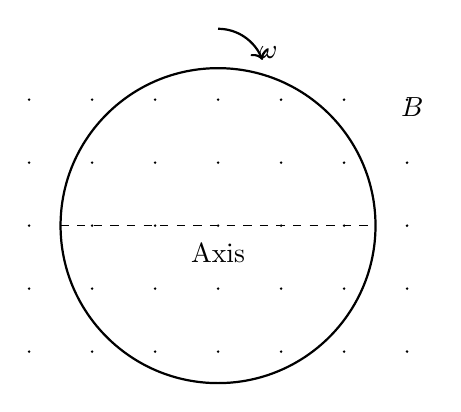
\begin{tikzpicture}[scale=1]

% Circle loop
\draw[thick] (0,0) circle (2);

% Diameter axis
\draw[dashed] (-2,0) -- (2,0);
\node[below] at (0,-0.1) {Axis};

% Magnetic field dots
\foreach \x in {-3,-2,...,3}
{
\foreach \y in {-2,-1,...,2}
{
\fill (\x*0.8,\y*0.8) circle (0.5pt);
}
}

\node[right] at (2.2,1.5) {$B$};

% Angular velocity arrow
\draw[->,thick] (0,2.5) arc (90:20:0.6);
\node[right] at (0.4,2.2) {$\omega$};

\end{tikzpicture}
\end{center}


A) $0$

B) $\dfrac{B\omega R^2}{2}$

C) $B\omega R^2$

D) $\dfrac{B\omega R}{2}$

%=========================================================
\item

A projectile of mass $m$ and charge $q$ is projected with speed $u$ at an angle $\theta$ to the horizontal in a region where a uniform magnetic field $B$ is perpendicular to the vertical plane of motion. 
Gravity acts downward and no electric field is present. 
Because of Lorentz force, the trajectory becomes a complex spatial curve instead of a simple parabola. 
Determine the nature of horizontal range measured along the ground plane.

A) $\dfrac{u^2\sin2\theta}{g}$

B) $\dfrac{u}{qB}\sin\theta$

C) undefined (no return)

D) depends on $B$

%=========================================================
\item

Two identical blocks each of mass $m$ are connected by a light spring of force constant $k$ and placed on a frictionless horizontal surface. 
A constant external force $F$ is applied to one block for a duration $t$ and then suddenly removed. 
During the force application, the center of mass accelerates while internal oscillations build up in the spring. 
Determine the maximum compression of the spring during the subsequent motion.

\begin{center}
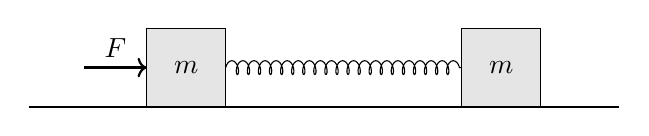
\begin{tikzpicture}[scale=1]

% Ground
\draw[thick] (-0.5,0) -- (7,0);

% Block 1
\draw[fill=gray!20] (1,0) rectangle (2,1);
\node at (1.5,0.5) {$m$};

% Block 2
\draw[fill=gray!20] (5,0) rectangle (6,1);
\node at (5.5,0.5) {$m$};

% Spring
\draw[decorate,decoration={coil,aspect=0.5,segment length=4pt}] 
(2,0.5) -- (5,0.5);

% Force arrow
\draw[->,thick] (0.2,0.5) -- (1,0.5);
\node[above] at (0.6,0.5) {$F$};

\end{tikzpicture}
\end{center}


A) $\dfrac{F^2t^2}{8mk}$

B) $\dfrac{F^2t^2}{4mk}$

C) $\dfrac{F^2t^2}{2mk}$

D) $\dfrac{F^2t^2}{mk}$

%=========================================================
\item 
A small particle is released from rest at the top of a smooth hemispherical bowl of radius $R$. 
As it slides down, the normal reaction decreases and eventually becomes zero at a certain angle $\theta$ measured from the vertical. 
Assume no friction and neglect rotational effects. 
Determine the value of $\cos\theta$ at the instant the particle loses contact with the surface.

\begin{center}
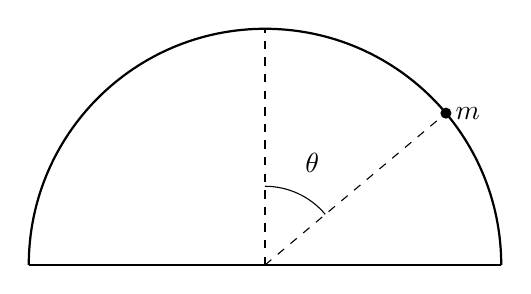
\begin{tikzpicture}[scale=1]

% Radius
\def\R{3}
\def\ang{50}

% Hemisphere
\draw[thick] (-\R,0) arc (180:0:\R);
\draw[thick] (-\R,0) -- (\R,0);

% Particle on surface
\coordinate (P) at ({\R*sin(\ang)},{\R*cos(\ang)});
\fill (P) circle (2pt);
\node[right] at (P) {$m$};

% Radius line
\draw[dashed] (0,0) -- (P);

% Vertical reference
\draw[dashed] (0,0) -- (0,\R);

% Angle theta
\draw (0,1) arc (90:{90-\ang}:1);
\node at (0.6,1.3) {$\theta$};

\end{tikzpicture}
\end{center}


A) $\dfrac{2}{3}$

B) $\dfrac{1}{2}$

C) $\dfrac{3}{4}$

D) $\dfrac{5}{6}$

%=========================================================
\item

A particle of mass $m$ attached to a spring executes simple harmonic motion with angular frequency $\omega_0$. 
A damping force proportional to velocity with coefficient $\beta$ is introduced such that the motion becomes underdamped. 
Total mechanical energy decreases exponentially with time due to dissipative losses. 
Determine the time at which total energy becomes exactly half of its initial value.

A) $\dfrac{\ln2}{2\beta}$

B) $\dfrac{\ln2}{\beta}$

C) $\dfrac{1}{2\beta}$

D) $\dfrac{1}{\beta}$

%=========================================================
\item

A parallel plate capacitor is half filled with a dielectric slab of dielectric constant $K$ while the remaining region contains air. 
The capacitor is first connected to a battery of voltage $V$ and then disconnected before the dielectric is slowly removed completely. 
Assume no fringing and negligible leakage. 
Determine the final potential difference across the capacitor.

A) $KV$

B) $\dfrac{2K}{K+1}V$

C) $\dfrac{K+1}{2}V$

D) unchanged

%=========================================================
\item

An electron moves in a circular orbit of radius $r$ around a nucleus due to Coulomb attraction. 
Assume classical circular motion and neglect relativistic effects. 
If the nuclear charge suddenly doubles while the electron’s angular momentum remains conserved, determine the new orbital radius.

A) $\dfrac{r}{2}$

B) $\dfrac{r}{4}$

C) $2r$

D) $4r$

%=========================================================
\item

In Young’s double slit experiment, a thin transparent sheet of refractive index $\mu$ and thickness $t$ is placed in front of one slit. 
Assume monochromatic light of wavelength $\lambda$ and screen distance $D \gg d$. 
The optical path difference introduced shifts the interference pattern without changing fringe spacing. 
Determine the number of fringe shifts produced on the screen.

A) $\dfrac{t(\mu-1)}{\lambda}$

B) $\dfrac{\lambda D}{dt}$

C) $\dfrac{t}{\mu}$

D) $\dfrac{t\mu}{\lambda}$

%=========================================================

\end{enumerate}

\end{document}